\documentclass[11pt,a4paper]{jsarticle}

\usepackage{amsmath,amssymb}
\usepackage{bm}
\usepackage{graphicx}
\usepackage{ascmac}
\usepackage{subfigure}
\newlength{\subfigwidth}
\newlength{\subfigcolsep}

\graphicspath{{./img/}}

\title{TPC-H performance measure}
\author{Keisuke Suzuki}

\begin{document}
\maketitle
\section{概要}
\begin{itemize}
 \item DBMS : PostgreSQL 9.2
 \item RAID0 : iodrive x8 (chunk size = 64KB)
 \item 各テーブルのprimary key上にB-tree indexを構築
 \item Scale Factor = 100
 \item shared buffer = 8GB
 \item 各クエリの実行時の状況をiostatとmpstatで1秒おきに監視
\end{itemize}

\section{Query実行中のsysの内訳分析}
\subsection{RAID0 (iodrive x8) read microbenchmark}
\begin{figure}[thbp]
 \setlength{\subfigwidth}{.5\linewidth}
 \addtolength{\subfigwidth}{-.5\subfigcolsep}
 \begin{minipage}[b]{\subfigwidth}
  \subfigure[IOPS]{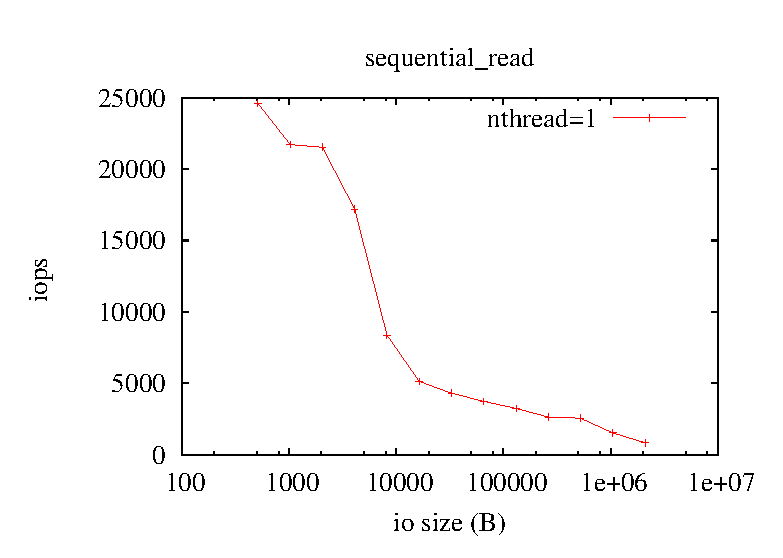
\includegraphics[width=75mm]{md0_sequential_read_iops_xiosize.eps}
  \label{fig:rmbench1}}
 \end{minipage}
  \begin{minipage}[b]{\subfigwidth}
    \subfigure[MBPS]{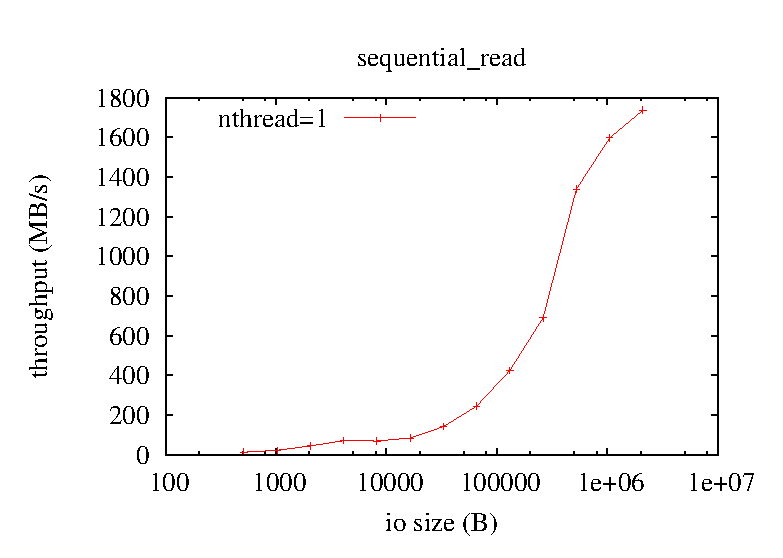
\includegraphics[width=75mm]{md0_sequential_read_throughput_xiosize.eps}
   \label{fig:rmbench2}}
  \end{minipage}
  \caption{read microbenchmark}
  \label{fig:rmbench}
\end{figure}

\begin{figure}[thbp]
 \begin{center}
  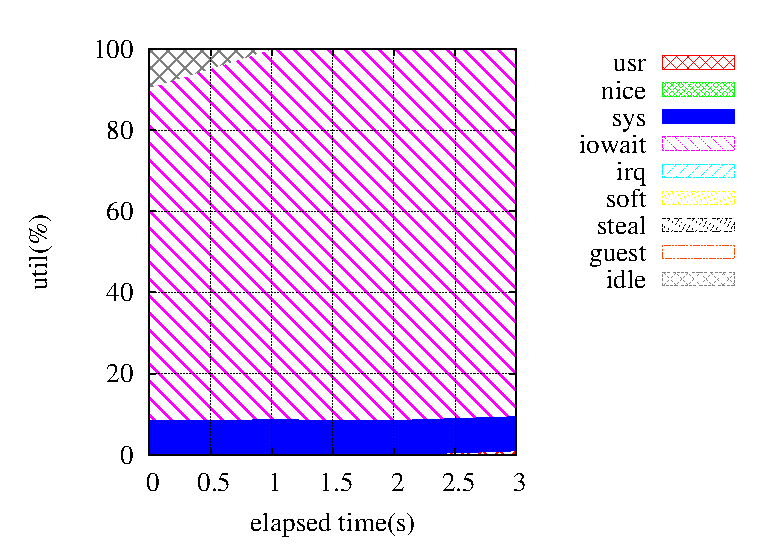
\includegraphics[width=110mm]{md0_io262144_thr1core8.eps}
 \end{center}
 \caption{cpu utilization (iosize = 256KB)}
 \label{fig:cpuutil256}
\end{figure}

\clearpage
\subsection{Query : count lineitem}
\begin{figure}[thbp]
 \begin{center}
  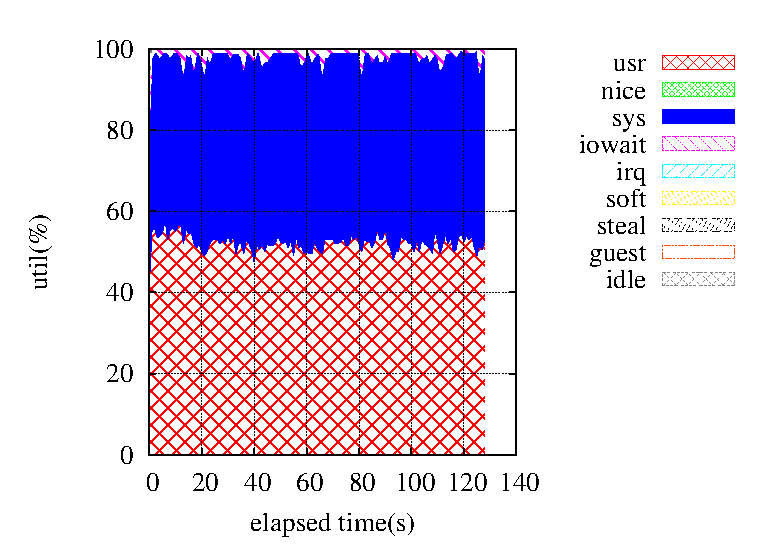
\includegraphics[width=110mm]{countlineitemcore1.eps}
 \end{center}
 \caption{cpu utilization}
 \label{fig:clinecpusys}
\end{figure}

\begin{figure}[thbp]
 \setlength{\subfigwidth}{.5\linewidth}
 \addtolength{\subfigwidth}{-.5\subfigcolsep}
 \begin{minipage}[b]{\subfigwidth}
  \subfigure[IOPS]{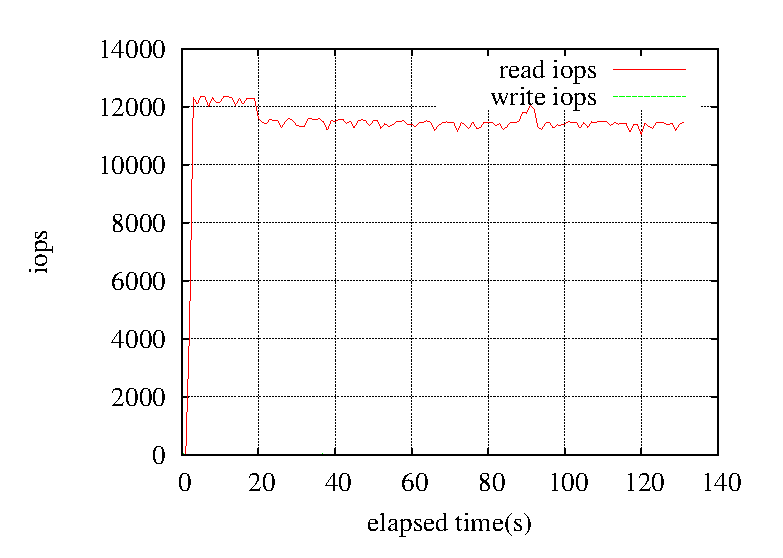
\includegraphics[width=75mm]{countlineitemiops.eps}
  \label{fig:clineiopssys}}
 \end{minipage}
  \begin{minipage}[b]{\subfigwidth}
    \subfigure[MBPS]{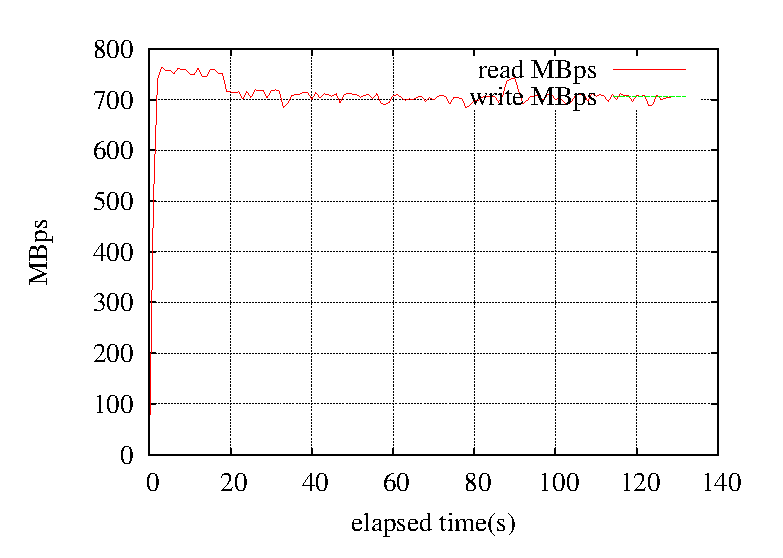
\includegraphics[width=75mm]{countlineitemmbps.eps}
   \label{fig:clinembpssys}}
  \end{minipage}
  \caption{IO spec}
  \label{fig:clinesys}
\end{figure}

\section{index scan on lineitem (l\_shipdate)}
\begin{figure}[thbp]
 \begin{center}
  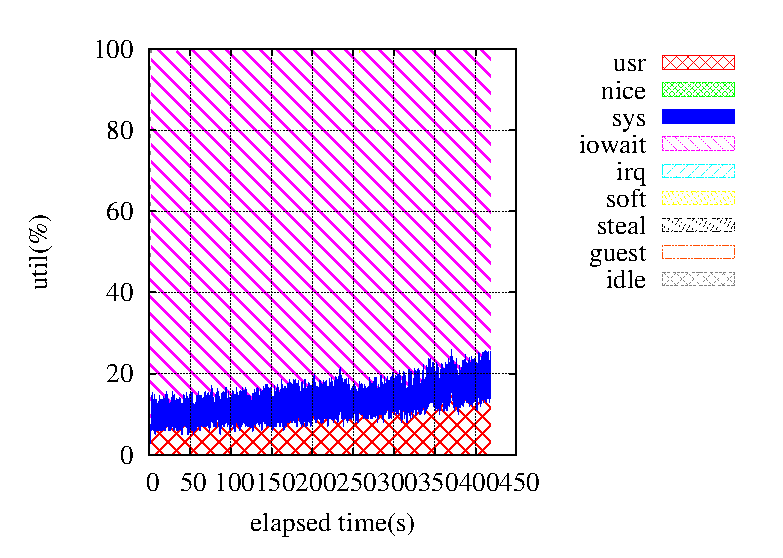
\includegraphics[width=110mm]{1_1core1.eps}
 \end{center}
 \caption{cpu utilization}
 \label{fig:1idxcpu}
\end{figure}

\begin{figure}[thbp]
 \setlength{\subfigwidth}{.5\linewidth}
 \addtolength{\subfigwidth}{-.5\subfigcolsep}
 \begin{minipage}[b]{\subfigwidth}
  \subfigure[IOPS]{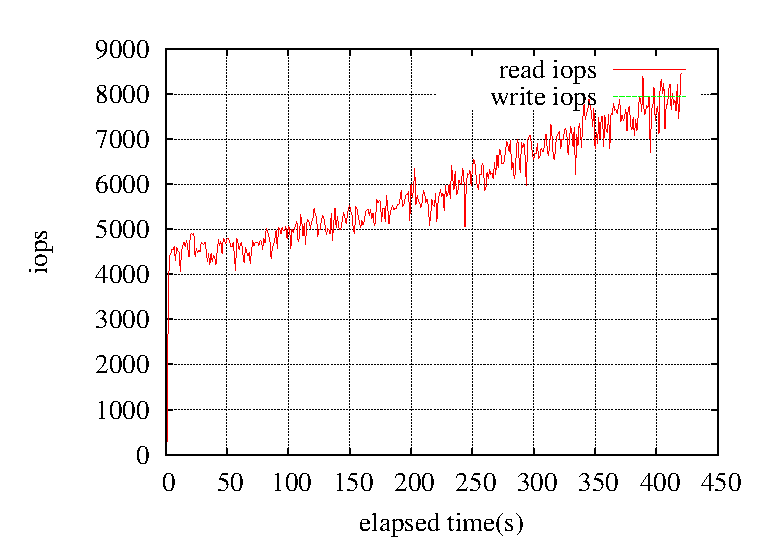
\includegraphics[width=75mm]{1_1iops.eps}
  \label{fig:1idxiops}}
 \end{minipage}
  \begin{minipage}[b]{\subfigwidth}
    \subfigure[MBPS]{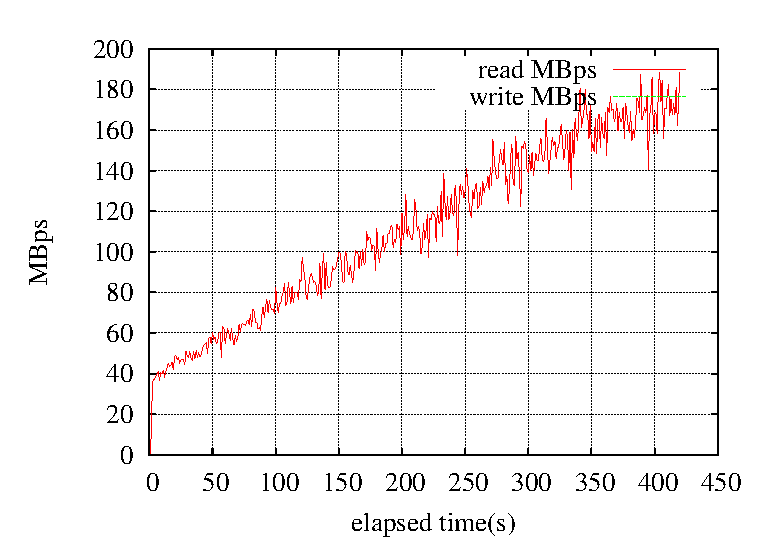
\includegraphics[width=75mm]{1_1mbps.eps}
   \label{fig:1idxmbps}}
  \end{minipage}
  \caption{IO spec}
  \label{fig:1idx}
\end{figure}

\end{document}
